% Provenance (never printed): cycle 2 "Explorer les organisations du monde ---
% identifier des paysages" (littoraux, massifs montagneux, campagnes, villes),
% see sources/book1/PROVENANCE.md. Book 1, grade 1, chapter 2.
\chapter{हमारे आसपास के भूदृश्य}\label{ch:g1:landscapes-around-us}

मिया और उसके दादाजी गाँव के पीछे वाली \omterm{def:g1:landscapes-around-us:landform}{पहाड़ी} पर चढ़कर बिलकुल ऊपर तक आ
गए हैं। चोटी पर वे साँस लेने के लिए घास पर बैठ जाते हैं, और देखते हैं।
नीचे गाँव की लाल छतें गिरजाघर के चारों ओर सटी हुई हैं। एक \omterm{def:g1:landscapes-around-us:water}{नदी} हरे और
पीले खेतों के बीच बल खाती हुई बहती है और एक पुल के नीचे से गुज़रती है।
अगली \omterm{def:g1:landscapes-around-us:landform}{पहाड़ी} पर एक घना जंगल है। और दूर, बहुत दूर, धरती के बिलकुल छोर पर,
नीले रंग की एक पतली-सी रेखा है।

``वह समुद्र है,'' दादाजी कहते हैं।

\omterm{def:g1:landscapes-around-us:landform}{पहाड़ी} की चोटी से मिया को पास और दूर जो कुछ भी दिखता है, वह सब एक
\omterm{def:g1:landscapes-around-us:landscape}{भूदृश्य} है।

\begin{omfigure}
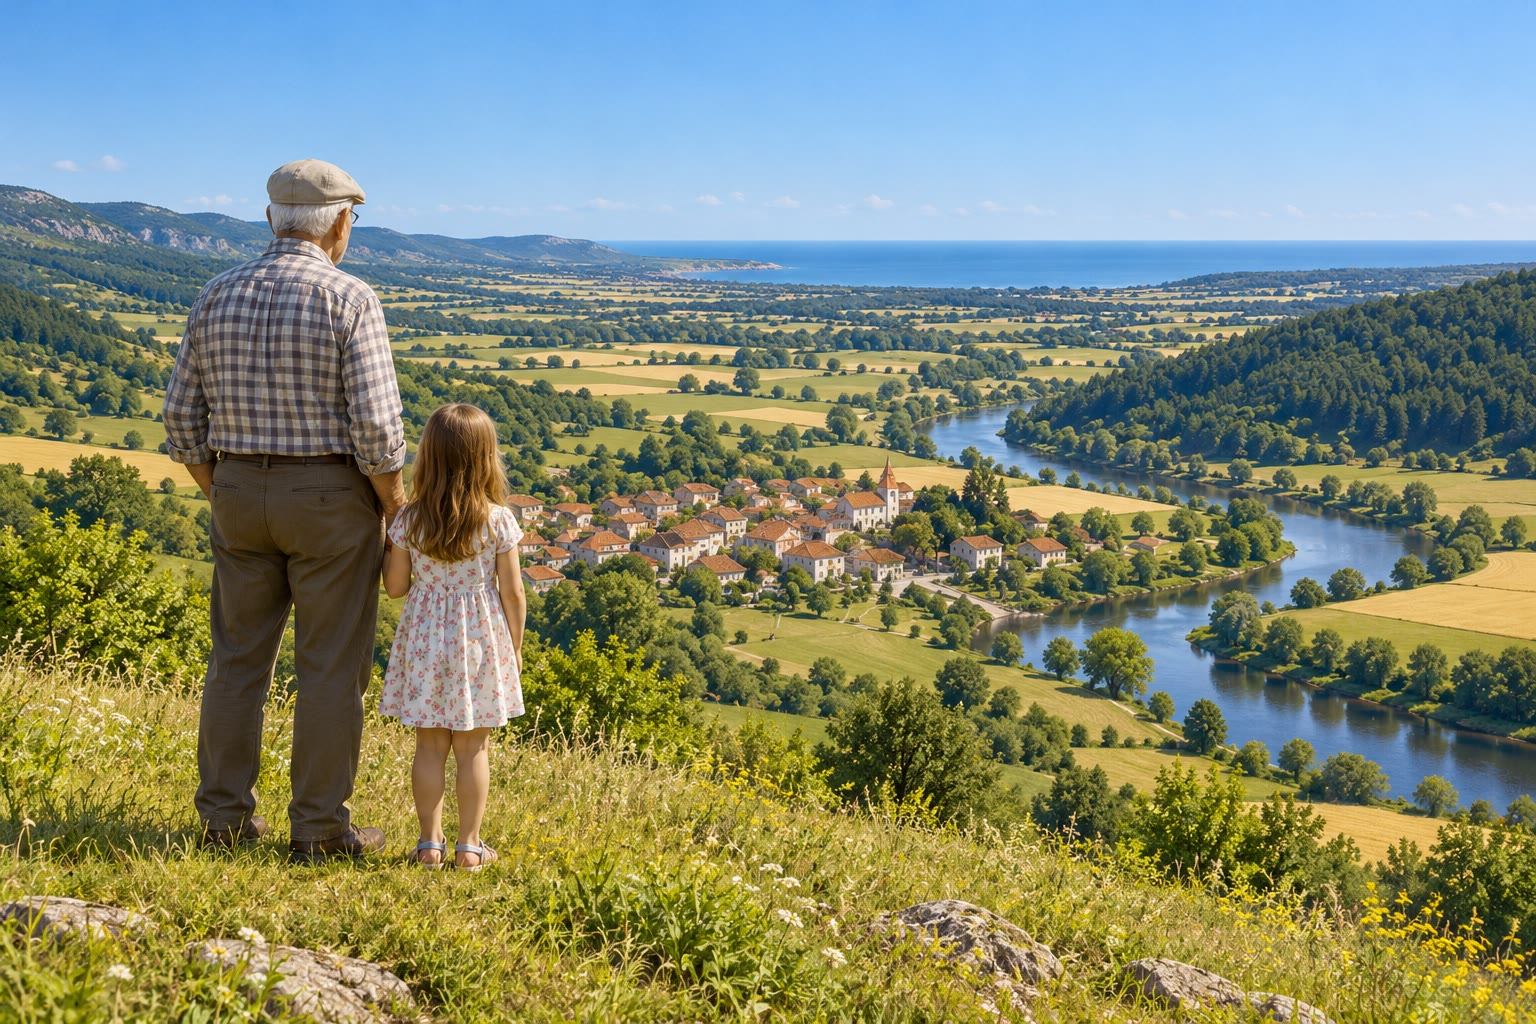
\includegraphics[width=0.72\linewidth]{images/book1/ai/g1-hilltop-view.jpg}

{\small \omterm{def:g1:landscapes-around-us:landform}{पहाड़ी} की चोटी से हमें पूरा \omterm{def:g1:landscapes-around-us:landscape}{भूदृश्य} दिखता है।}
\end{omfigure}

\section{भूदृश्य क्या है?}

\begin{definition}[भूदृश्य]\label{def:g1:landscapes-around-us:landscape}
जहाँ हम खड़े हैं वहाँ से दूर क्षितिज तक, एक नज़र में ज़मीन का जितना कुछ
हमें दिखता है, वह सब \emph{भूदृश्य}\index{भूदृश्य} है: ज़मीन का आकार,
पानी, पेड़-पौधे, और लोगों की बनाई चीज़ें।
\end{definition}

\omterm{def:g1:landscapes-around-us:landscape}{भूदृश्य} के कुछ भाग पास होते हैं और कुछ दूर। जो भाग हमारे सबसे पास है, वह
हमें दिखने वाले दृश्य में सबसे नीचे होता है; वह बड़ा दिखता है और उसकी
बारीकियाँ दिखती हैं। दूर वाला भाग ऊपर, आसमान के पास होता है; वह छोटा और
फीका दिखता है।

\begin{omfigure}
\begin{tikzpicture}[x=1cm, y=1cm]
  \fill[ocBlue!12] (0,0) rectangle (10,5);
  % background: far hills
  \fill[black!18] (0,3.0) -- (1.5,3.6) -- (3,3.3) -- (5,3.9) -- (7,3.4) -- (8.5,3.8) -- (10,3.3) -- (10,2.9) -- (0,2.9) -- cycle;
  % middle: hills and fields
  \fill[green!35!omLithAlluv] (0,1.6) -- (2,2.4) -- (4,2.1) -- (6,2.7) -- (8,2.2) -- (10,2.5) -- (10,1.5) -- (0,1.5) -- cycle;
  \fill[green!25!omLithAlluv] (0,1.5) rectangle (10,2.95);
  \fill[green!35!omLithAlluv] (0,2.95) -- (2,3.1) -- (4,2.95) -- (6,3.25) -- (8,3.0) -- (10,3.1) -- (10,2.9) -- (0,2.9) -- cycle;
  \foreach \x in {5.6,5.9,6.2} \fill[red!55] (\x,2.25) -- ++(0.12,0.15) -- ++(0.12,-0.15) -- cycle;
  \foreach \x in {5.6,5.9,6.2} \fill[white] (\x+0.03,2.1) rectangle ++(0.18,0.15);
  % foreground
  \fill[green!55!black!60] (0,0) rectangle (10,1.5);
  \foreach \x in {0.8,2.1,8.6} {
    \fill[brown!70!black] (\x-0.06,0.4) rectangle (\x+0.06,0.9);
    \fill[green!45!black] (\x,1.15) circle (0.38);
  }
  % band borders and labels
  \draw[white, line width=1pt, dashed] (0,1.5) -- (10,1.5);
  \draw[white, line width=1pt, dashed] (0,2.95) -- (10,2.95);
  \node[font=\small\bfseries, fill=white, fill opacity=0.8, text opacity=1, inner sep=2pt] at (5,0.6) {अग्रभूमि: पास, बड़ी, बहुत-सी बारीकियाँ};
  \node[font=\small\bfseries, fill=white, fill opacity=0.8, text opacity=1, inner sep=2pt] at (2.7,2.2) {मध्यभूमि};
  \node[font=\small\bfseries, fill=white, fill opacity=0.8, text opacity=1, inner sep=2pt] at (5,4.4) {पृष्ठभूमि: दूर, छोटी, फीकी};
\end{tikzpicture}

{\small तीन पट्टियों में देखा गया एक \omterm{def:g1:landscapes-around-us:landscape}{भूदृश्य}: नीचे अग्रभूमि, फिर मध्यभूमि,
और आसमान से सटी पृष्ठभूमि।}
\label{fig:g1:landscapes-around-us:bands}
\end{omfigure}

\section{ज़मीन के आकार}

ज़मीन हर जगह समतल नहीं होती। कहीं वह आसमान में ऊँची उठ जाती है; कहीं वह
लंबे गड्ढों में नीचे चली जाती है; और कहीं जहाँ तक नज़र जाए, समतल रहती है।
हम हर आकार को एक नाम देते हैं।

\begin{definition}[स्थलरूप]\label{def:g1:landscapes-around-us:landform}
ज़मीन की सतह का कोई आकार \emph{स्थलरूप}\index{स्थलरूप} कहलाता है।
\begin{itemize}
  \item \emph{पर्वत}\index{पर्वत} बहुत ऊँचा स्थलरूप है जिसकी ढलानें खड़ी
        होती हैं; उसके सबसे ऊपरी भाग को शिखर कहते हैं। सबसे ऊँचे पर्वतों
        की चोटी पर गर्मियों में भी बर्फ़ रहती है।
  \item \emph{पहाड़ी}\index{पहाड़ी} ऐसा स्थलरूप है जो अपने आसपास की ज़मीन से
        ऊपर उठा होता है, पर पर्वत से नीचा और गोल होता है।
  \item \emph{घाटी}\index{घाटी} पहाड़ियों या पर्वतों के बीच का एक लंबा, नीचा
        गड्ढा है; उसकी तली में अक्सर एक \omterm{def:g1:landscapes-around-us:water}{नदी} बहती है।
  \item \emph{मैदान}\index{मैदान} ज़मीन का एक चौड़ा, समतल और नीचा फैलाव है।
\end{itemize}
\end{definition}

\begin{omfigure}
\begin{tikzpicture}[x=1cm, y=1cm]
  \fill[ocBlue!10] (0,0) rectangle (12.4,4.6);
  % sea
  \fill[omSea] (10.2,0) rectangle (12.4,0.55);
  % land profile: mountains, valley, hill, plain, coast
  \fill[omLithAlluv!80!green] (0,0) -- (0,2.2) -- (0.9,3.3) -- (1.5,3.0) -- (2.2,4.1)
     -- (2.9,2.6) -- (3.6,1.2) -- (3.9,0.9) -- (4.2,1.2) -- (5.0,2.0) -- (5.7,2.2)
     -- (6.4,1.6) -- (7.0,0.95) -- (8.0,0.8) -- (9.5,0.7) -- (10.2,0.6) -- (10.4,0.55)
     -- (10.4,0) -- cycle;
  \draw[black!60, line width=0.6pt] (0,2.2) -- (0.9,3.3) -- (1.5,3.0) -- (2.2,4.1)
     -- (2.9,2.6) -- (3.6,1.2) -- (3.9,0.9) -- (4.2,1.2) -- (5.0,2.0) -- (5.7,2.2)
     -- (6.4,1.6) -- (7.0,0.95) -- (8.0,0.8) -- (9.5,0.7) -- (10.2,0.6) -- (10.4,0.55);
  % snow caps
  \fill[white, draw=black!50, line width=0.3pt] (1.95,3.72) -- (2.2,4.1) -- (2.45,3.72) -- (2.3,3.78) -- (2.2,3.68) -- (2.08,3.78) -- cycle;
  \fill[white, draw=black!50, line width=0.3pt] (0.72,3.08) -- (0.9,3.3) -- (1.05,3.15) -- (0.9,3.12) -- cycle;
  % river in the valley
  \fill[omSea!90!black] (3.75,0.92) rectangle (4.05,0.98);
  % lake on the plain
  \fill[omSea] (7.6,0.82) ellipse (0.5 and 0.07);
  % village on the plain
  \foreach \x in {8.6,8.85,9.1} {
    \fill[white, draw=black!50, line width=0.3pt] (\x,0.74) rectangle ++(0.18,0.16);
    \fill[red!60] (\x-0.02,0.9) -- ++(0.11,0.12) -- ++(0.11,-0.12) -- cycle;
  }
  % labels
  \node[font=\small, above] at (2.2,4.12) {पर्वत};
  \node[font=\small, above] at (5.6,2.25) {पहाड़ी};
  \node[font=\small] at (3.9,1.85) {घाटी};
  \node[font=\small, above] at (8.2,1.5) {मैदान};
  \draw[black!60, thin] (8.2,1.5) -- (8.2,0.85);
  \node[font=\small, align=center] at (11.3,1.4) {समुद्र};
  \node[font=\scriptsize, below=2pt, fill=white, fill opacity=0.8, text opacity=1, inner sep=1pt] at (7.6,0.35) {झील};
  \draw[black!60, thin] (7.6,0.45) -- (7.6,0.78);
  \node[font=\scriptsize, below=2pt, fill=white, fill opacity=0.8, text opacity=1, inner sep=1pt] at (10.3,0.35) {तट};
  \node[font=\scriptsize, fill=white, fill opacity=0.8, text opacity=1, inner sep=1pt] at (3.9,0.2) {नदी};
  \draw[black!60, thin] (3.9,0.32) -- (3.9,0.88);
\end{tikzpicture}

{\small \omterm{def:g1:landscapes-around-us:landform}{पर्वतों} से समुद्र तक ज़मीन के आकार, बगल से देखे हुए (ऊँचाइयाँ असल से
बहुत ज़्यादा ऊँची बनाई गई हैं)।}
\label{fig:g1:landscapes-around-us:profile}
\end{omfigure}

\begin{omfigure}
\begin{minipage}[b]{0.49\linewidth}\centering
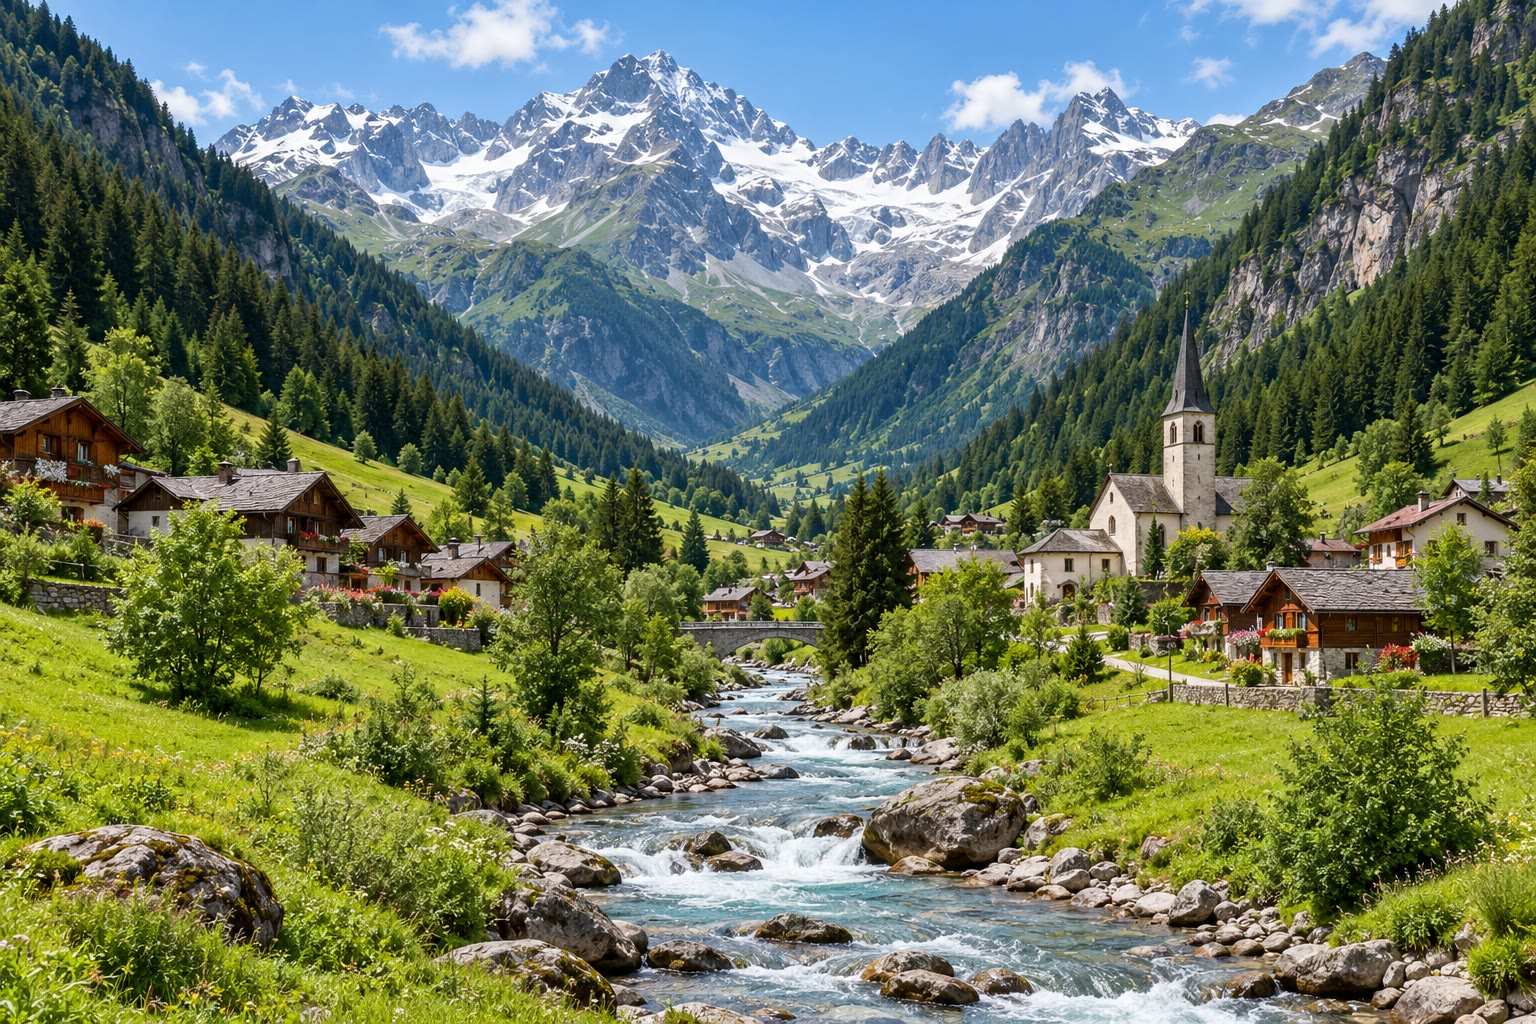
\includegraphics[width=\linewidth]{images/book1/ai/g1-mountain-village.jpg}

{\small \omterm{def:g1:landscapes-around-us:landform}{पर्वत}, और उनकी \omterm{def:g1:landscapes-around-us:landform}{घाटी} में बसा एक गाँव।}
\end{minipage}\hfill
\begin{minipage}[b]{0.49\linewidth}\centering
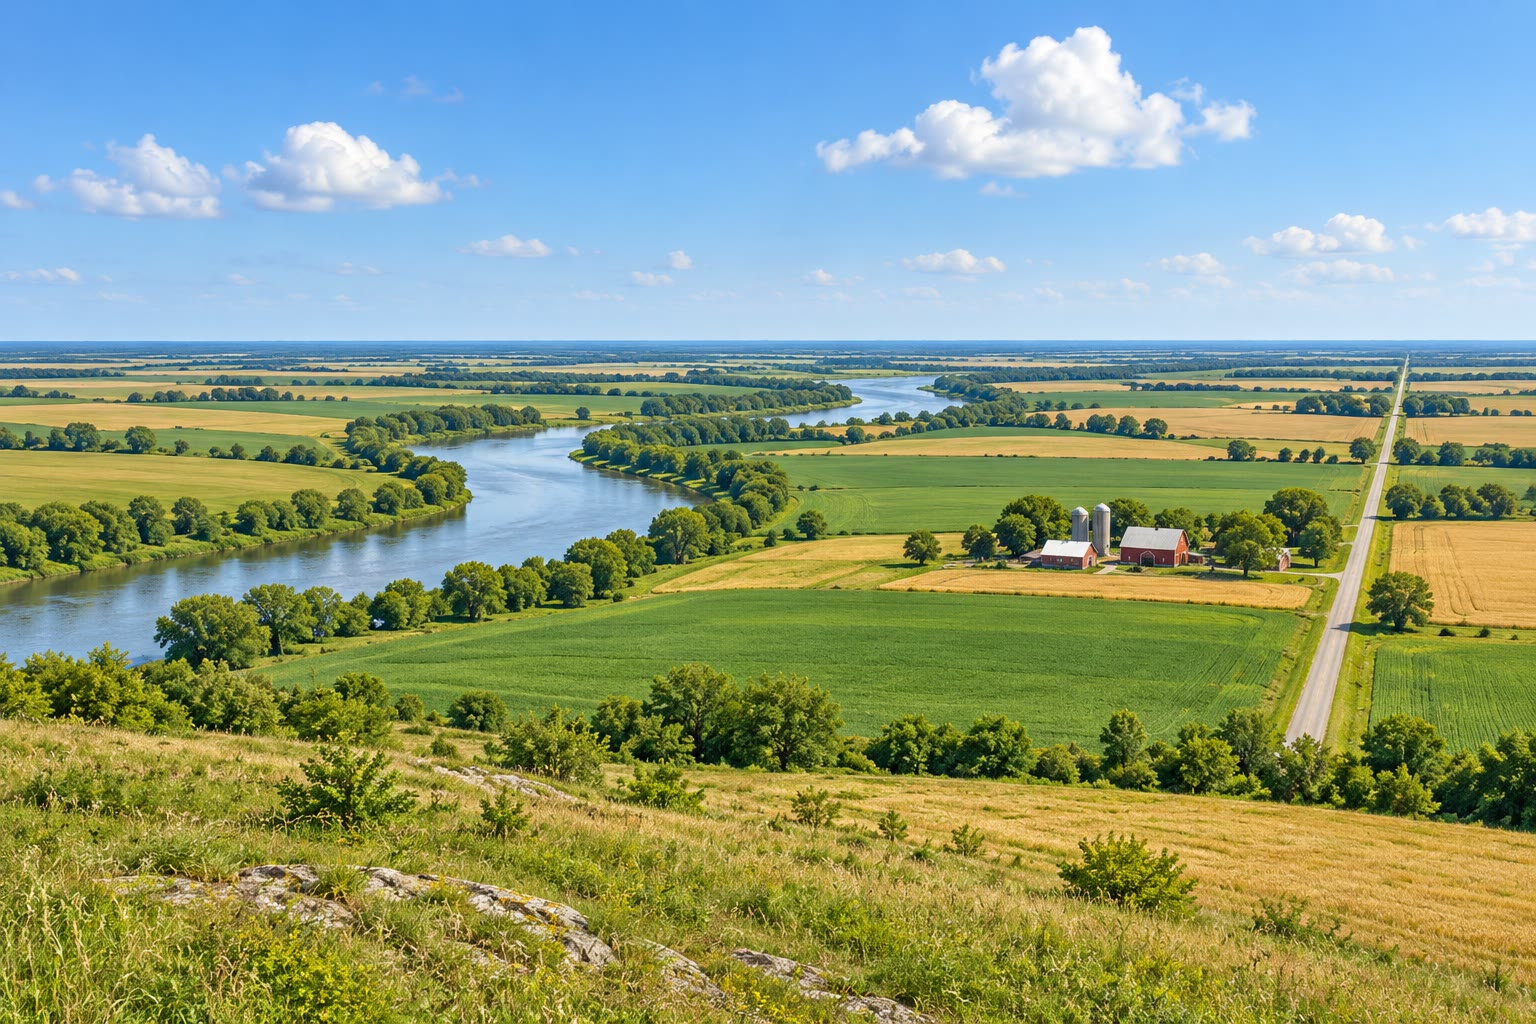
\includegraphics[width=\linewidth]{images/book1/ai/g1-plain-river.jpg}

{\small एक \omterm{def:g1:landscapes-around-us:landform}{मैदान}, जिसमें एक \omterm{def:g1:landscapes-around-us:water}{नदी} और खेत हैं।}
\end{minipage}
\end{omfigure}

\begin{example}[पर्वत या पहाड़ी?]\label{ex:g1:landscapes-around-us:mountain-hill}
ऐसी कोई ठीक-ठीक ऊँचाई नहीं है जिस पर पहुँचकर \omterm{def:g1:landscapes-around-us:landform}{पहाड़ी} \omterm{def:g1:landscapes-around-us:landform}{पर्वत} बन जाती हो। हम
आकार देखते हैं: \omterm{def:g1:landscapes-around-us:landform}{पर्वत} ऊँचा और खड़ा होता है, अक्सर पथरीला, कभी-कभी चोटी
पर बर्फ़ के साथ; \omterm{def:g1:landscapes-around-us:landform}{पहाड़ी} नीची और गोल होती है, अक्सर घास, खेतों या
झाड़ियों-पेड़ों से ढकी, और हम थोड़ी ही देर में चलकर उसकी चोटी तक पहुँच
सकते हैं।
\end{example}

\section{भूदृश्य में पानी}

ज़्यादातर \omterm{def:g1:landscapes-around-us:landscape}{भूदृश्यों} में पानी होता है। वह \omterm{def:g1:landscapes-around-us:landform}{पहाड़ियों} और \omterm{def:g1:landscapes-around-us:landform}{पर्वतों} से नीचे
बहता है, गड्ढों में इकट्ठा होता है, और समुद्र तक पहुँचता है।

\begin{definition}[भूदृश्य में पानी]\label{def:g1:landscapes-around-us:water}
\emph{नदी}\index{नदी} वह पानी है जो एक लंबी धारा में हर समय बहता रहता
है, ऊँची ज़मीन से नीचे किसी झील या समुद्र तक। \emph{झील}\index{झील}
चारों ओर ज़मीन से घिरा पानी का एक बड़ा फैलाव है। \emph{तट}\index{तट} वह
जगह है जहाँ ज़मीन समुद्र से मिलती है।
\end{definition}

\begin{omfigure}
\begin{minipage}[b]{0.49\linewidth}\centering
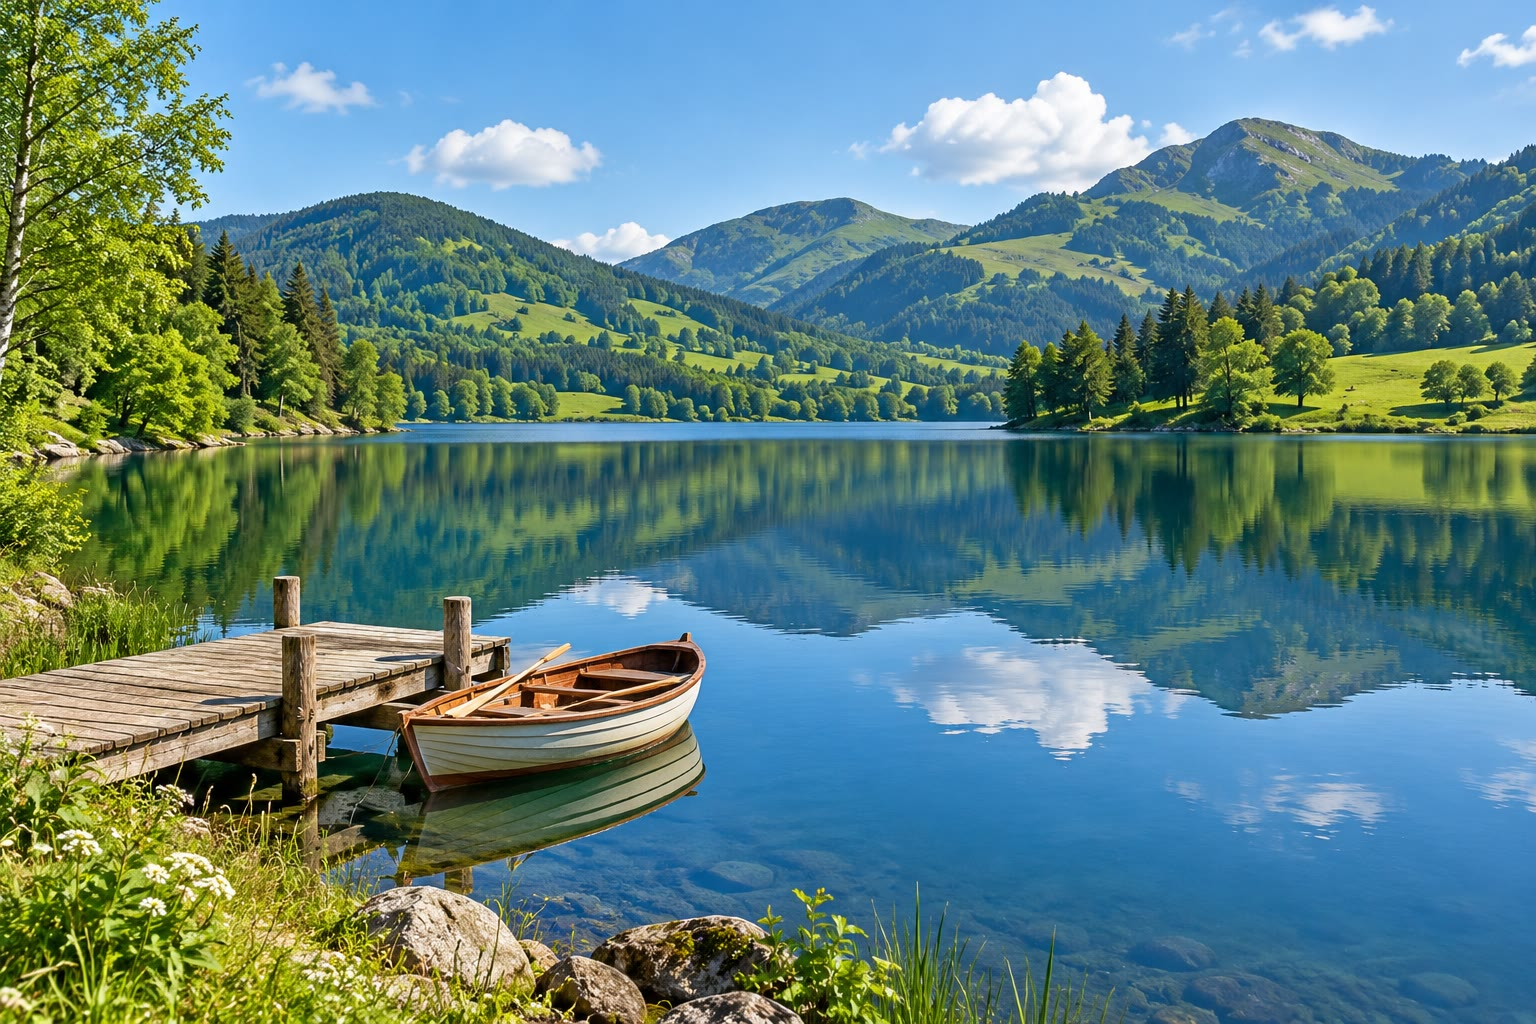
\includegraphics[width=\linewidth]{images/book1/ai/g1-lake-hills.jpg}

{\small \omterm{def:g1:landscapes-around-us:landform}{पहाड़ियों} के बीच एक \omterm{def:g1:landscapes-around-us:water}{झील}।}
\end{minipage}\hfill
\begin{minipage}[b]{0.49\linewidth}\centering
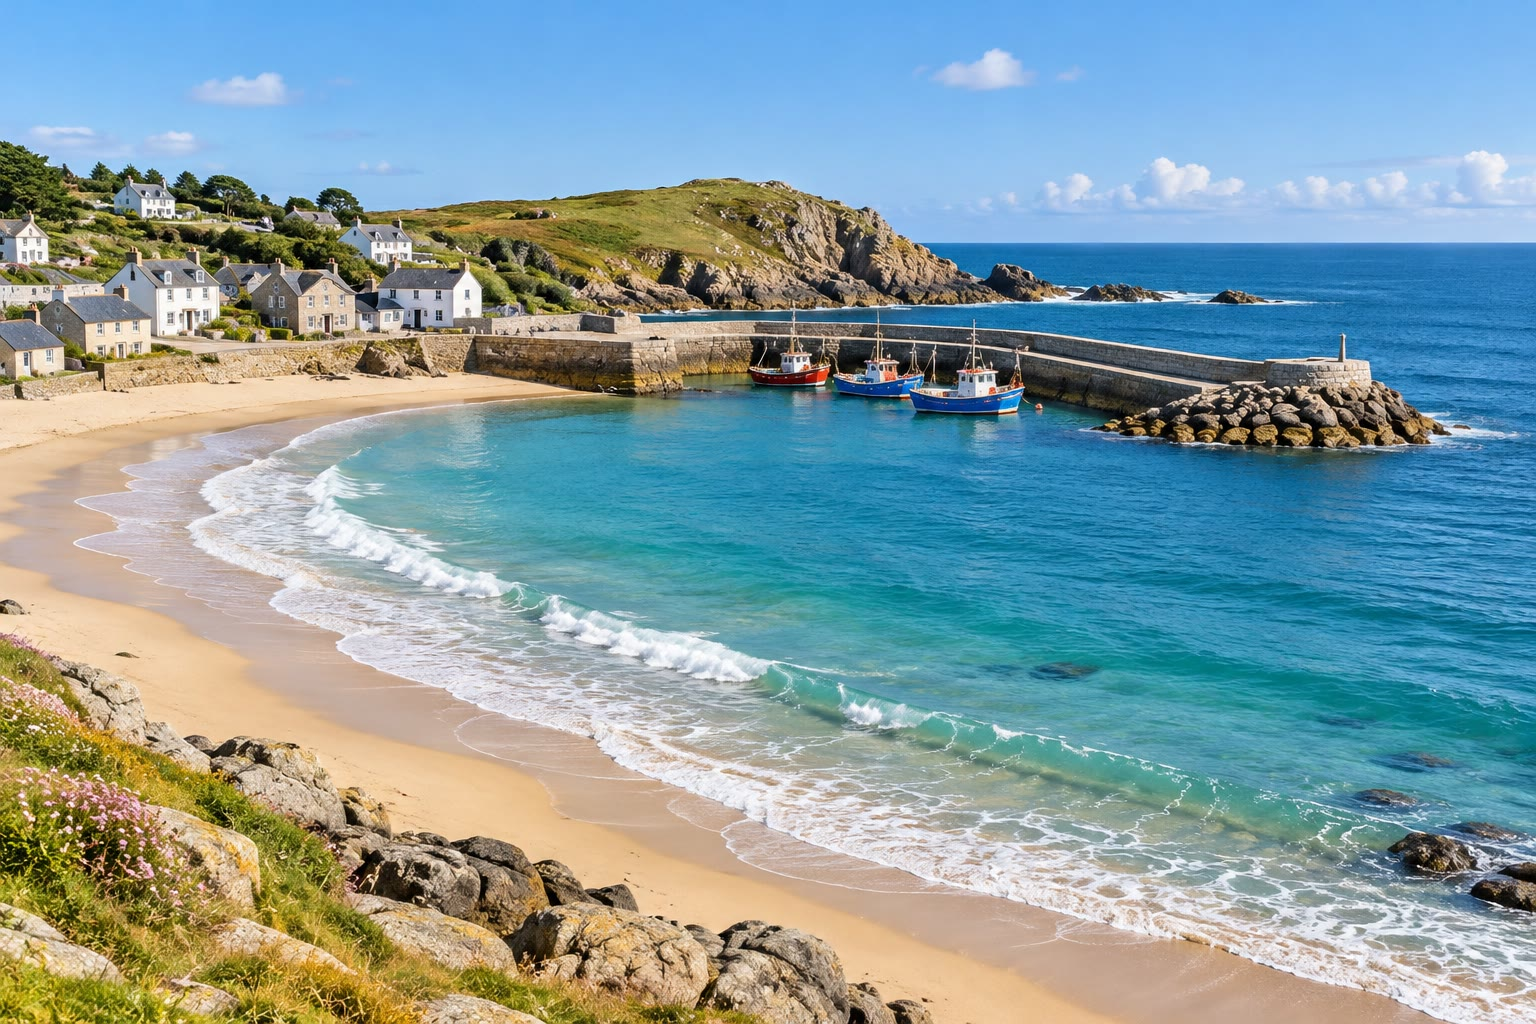
\includegraphics[width=\linewidth]{images/book1/ai/g1-coast-harbour.jpg}

{\small एक \omterm{def:g1:landscapes-around-us:water}{तट}: रेतीला किनारा, चट्टानें और एक बंदरगाह।}
\end{minipage}
\end{omfigure}

\begin{remark}[पानी हमेशा ढलान की ओर बहता है]\label{rem:g1:landscapes-around-us:downhill}
\omterm{def:g1:landscapes-around-us:water}{नदी} हमेशा ऊँची ज़मीन से नीची ज़मीन की ओर बहती है। इसीलिए \omterm{def:g1:landscapes-around-us:water}{नदियाँ} \omterm{def:g1:landscapes-around-us:landform}{घाटियों}
की तली में बहती हैं, और इसीलिए आख़िर में वे किसी \omterm{def:g1:landscapes-around-us:water}{झील} या समुद्र तक पहुँचती
हैं, जो अपने आसपास की ज़मीन से नीचे होते हैं।
\end{remark}

\section{प्राकृतिक भाग और बनाए गए भाग}

\omterm{def:g1:landscapes-around-us:landscape}{भूदृश्य} के कुछ भाग लोगों के आने से पहले भी वहाँ थे: \omterm{def:g1:landscapes-around-us:landform}{पर्वत}, \omterm{def:g1:landscapes-around-us:water}{नदियाँ},
जंगल। दूसरे भाग लोगों ने बनाए: घर, सड़कें, पुल, खेत।

\begin{definition}[प्राकृतिक और मानव-निर्मित भाग]\label{def:g1:landscapes-around-us:natural-built}
\omterm{def:g1:landscapes-around-us:landscape}{भूदृश्य} का \emph{प्राकृतिक तत्व}\index{प्राकृतिक तत्व} वह भाग है जिसे
लोगों ने नहीं बनाया: \omterm{def:g1:landscapes-around-us:landform}{पर्वत}, \omterm{def:g1:landscapes-around-us:water}{नदी}, \omterm{def:g1:landscapes-around-us:water}{झील}, जंगल, रेतीला किनारा।
\emph{मानव-निर्मित तत्व}\index{मानव-निर्मित तत्व} वह भाग है जिसे लोगों ने
बनाया या गढ़ा है: घर, सड़क, पुल, बंदरगाह, खेत, बग़ीचा।
\end{definition}

\begin{omfigure}
\begin{tikzpicture}[x=1cm, y=1cm]
  \node[draw=omDef!80!black, fill=omDef!10, rounded corners, text width=5.2cm,
        align=left, minimum height=3.2cm, anchor=north] (n) at (0,0)
    {\textbf{प्राकृतिक}\\[2pt] पर्वत\\ पहाड़ी\\ घाटी\\ नदी\\ झील\\ जंगल\\ रेतीला किनारा};
  \node[draw=omMeth!80!black, fill=omMeth!10, rounded corners, text width=5.2cm,
        align=left, minimum height=3.2cm, anchor=north] (b) at (6,0)
    {\textbf{लोगों के बनाए}\\[2pt] घर\\ गिरजाघर\\ सड़क\\ पुल\\ बंदरगाह\\ खेत\\ बग़ीचा};
\end{tikzpicture}

{\small मिया के \omterm{def:g1:landscapes-around-us:landscape}{भूदृश्य} के भागों को छाँटना। खेत मानव-निर्मित है: लोगों ने
ज़मीन साफ़ की और उसमें फ़सल बोई।}
\label{fig:g1:landscapes-around-us:sort}
\end{omfigure}

\section{भूदृश्य बदलते हैं}

\omterm{def:g1:landscapes-around-us:landscape}{भूदृश्य} हमेशा एक जैसा नहीं रहता। कुछ बदलाव जल्दी होते हैं, और कुछ इतने
धीमे कि किसी को पूरी ज़िंदगी में दिखाई नहीं देते।
\begin{itemize}
  \item \textbf{ऋतुओं के साथ:} जुताई के बाद खेत भूरे होते हैं, वसंत में
        हरे, कटाई से पहले सुनहरे; पतझड़ में पेड़ों की पत्तियाँ झड़ जाती हैं;
        सर्दियों में बर्फ़ सब कुछ ढक सकती है।
  \item \textbf{लोगों के कारण:} गाँव बढ़कर क़स्बा बन जाता है; खेत बनाने के
        लिए जंगल काट दिया जाता है; एक नई सड़क और एक पुल \omterm{def:g1:landscapes-around-us:landform}{घाटी} को पार करते
        हैं।
  \item \textbf{पानी और \omterm{def:g1:watching-the-weather:weather}{मौसम} के कारण:} किसी बड़े तूफ़ान के बाद \omterm{def:g1:landscapes-around-us:water}{नदी} अपना
        तल छोड़कर कुछ दिनों के लिए खेतों पर फैल सकती है; \omterm{def:g1:landscapes-around-us:water}{तट} पर लहरें
        धीरे-धीरे चट्टानों को घिस देती हैं।
\end{itemize}

\begin{omfigure}
\begin{tikzpicture}[x=1cm, y=1cm]
  \foreach \k/\t in {0/बहुत पहले, 1/आज} {
  \begin{scope}[shift={(\k*6.4,0)}]
    \fill[ocBlue!8] (0,0) rectangle (5.8,3.4);
    \fill[green!30!omLithAlluv] (0,0) rectangle (5.8,1.9);
    % river
    \fill[omSea] (0,0.55) .. controls (1.5,0.9) and (2.5,0.2) .. (5.8,0.6)
       -- (5.8,0.85) .. controls (2.5,0.45) and (1.5,1.15) .. (0,0.8) -- cycle;
    % hill
    \fill[green!45!black!55] (2.8,1.9) .. controls (3.8,3.1) and (4.8,3.1) .. (5.8,2.2) -- (5.8,1.9) -- cycle;
    \ifnum\k=0
      % forest everywhere, a few houses
      \foreach \x in {0.4,0.9,1.4,1.9,2.4,4.3,4.8,5.3}
        \fill[green!40!black] (\x,1.45) circle (0.22);
      \foreach \x in {3.4,3.75} {
        \fill[white, draw=black!50, line width=0.3pt] (\x,1.15) rectangle ++(0.24,0.2);
        \fill[red!60] (\x-0.03,1.35) -- ++(0.15,0.14) -- ++(0.15,-0.14) -- cycle; }
    \else
      % fields, many houses, a road and a bridge
      \foreach \x/\c in {0.1/yellow!60, 1.3/green!55, 4.5/yellow!45}
        \fill[\c] (\x,1.05) rectangle ++(1.1,0.5);
      \fill[black!35] (2.65,0) rectangle (2.95,1.9);
      \fill[black!55] (2.55,0.5) rectangle (3.05,0.9);
      \foreach \x in {3.2,3.55,3.9} \foreach \y in {1.1,1.45} {
        \fill[white, draw=black!50, line width=0.3pt] (\x,\y) rectangle ++(0.24,0.2);
        \fill[red!60] (\x-0.03,\y+0.2) -- ++(0.15,0.14) -- ++(0.15,-0.14) -- cycle; }
      \foreach \x in {4.6,5.2} \fill[green!40!black] (\x,2.35) circle (0.2);
    \fi
    \node[font=\small\bfseries] at (2.9,-0.3) {\t};
  \end{scope}}
\end{tikzpicture}

{\small वही \omterm{def:g1:landscapes-around-us:landform}{घाटी} बहुत पहले और आज। \omterm{def:g1:landscapes-around-us:landform}{पहाड़ी} और \omterm{def:g1:landscapes-around-us:water}{नदी} अपनी जगह से नहीं हटीं;
लोगों ने ज़्यादातर जंगल काट दिया, खेत बनाए, और ज़्यादा घर, एक सड़क और
एक पुल बनाया।}
\label{fig:g1:landscapes-around-us:change}
\end{omfigure}

\begin{example}[शहर और गाँव-देहात]\label{ex:g1:landscapes-around-us:town}
शहर में लगभग सब कुछ जो हम देखते हैं, बनाया गया है: गलियाँ, घर, दुकानें,
पुल, पार्क। देहात में हमें ज़्यादातर खेत, जंगल और चरागाह दिखते हैं, और
कुछ फ़ार्म और गाँव। दोनों \omterm{def:g1:landscapes-around-us:landscape}{भूदृश्य} हैं। किसी बड़े शहर के बीचोंबीच भी
ज़मीन के आकार बने रहते हैं: शहर के बीच से एक \omterm{def:g1:landscapes-around-us:water}{नदी} गुज़रती है, और कुछ
गलियाँ \omterm{def:g1:landscapes-around-us:landform}{पहाड़ी} पर चढ़ती हैं।
\end{example}

\section{भूदृश्य का वर्णन करना}

\begin{method}[चार चरणों में भूदृश्य का वर्णन]\label{met:g1:landscapes-around-us:describe}
किसी \omterm{def:g1:landscapes-around-us:landform}{पहाड़ी} की चोटी से या किसी चित्र से \omterm{def:g1:landscapes-around-us:landscape}{भूदृश्य} का वर्णन करने के लिए:
\begin{enumerate}
  \item \textbf{उसे तीन पट्टियों में बाँटो:} अग्रभूमि, मध्यभूमि और
        पृष्ठभूमि।
  \item \textbf{ज़मीन के आकारों के नाम बताओ:} \omterm{def:g1:landscapes-around-us:landform}{पर्वत}, \omterm{def:g1:landscapes-around-us:landform}{पहाड़ियाँ}, \omterm{def:g1:landscapes-around-us:landform}{घाटियाँ},
        \omterm{def:g1:landscapes-around-us:landform}{मैदान}।
  \item \textbf{पानी ढूँढो:} \omterm{def:g1:landscapes-around-us:water}{नदी}, \omterm{def:g1:landscapes-around-us:water}{झील}, समुद्र और उसका \omterm{def:g1:landscapes-around-us:water}{तट}।
  \item \textbf{लोगों की बनाई चीज़ें ढूँढो:} घर, सड़कें, पुल,
        खेत।
\end{enumerate}
\end{method}

\begin{example}[मिया का भूदृश्य]\label{ex:g1:landscapes-around-us:mia}
अग्रभूमि में: \omterm{def:g1:landscapes-around-us:landform}{पहाड़ी} की चोटी की घास। मध्यभूमि में: एक \omterm{def:g1:landscapes-around-us:landform}{घाटी} जिसमें एक
\omterm{def:g1:landscapes-around-us:water}{नदी}, एक पुल और एक गाँव है, उसके चारों ओर खेत, और अगली \omterm{def:g1:landscapes-around-us:landform}{पहाड़ी} पर एक
जंगल। पृष्ठभूमि में: एक \omterm{def:g1:landscapes-around-us:landform}{मैदान} और, धरती के छोर पर, \omterm{def:g1:landscapes-around-us:water}{तट} और समुद्र।
प्राकृतिक: \omterm{def:g1:landscapes-around-us:landform}{पहाड़ियाँ}, \omterm{def:g1:landscapes-around-us:landform}{घाटी}, \omterm{def:g1:landscapes-around-us:water}{नदी}, जंगल, समुद्र। मानव-निर्मित: गाँव,
गिरजाघर, पुल, खेत।
\end{example}

\section{अभ्यास}

\begin{exercise}[$\star$]\label{exo:g1:landscapes-around-us:1}
इस अध्याय में तुमने ज़मीन के जो चार आकार सीखे, उनके नाम बताओ।
\end{exercise}

\begin{exercise}[$\star$]\label{exo:g1:landscapes-around-us:2}
कौन ज़्यादा ऊँचा और ज़्यादा खड़ा है: \omterm{def:g1:landscapes-around-us:landform}{पहाड़ी} या \omterm{def:g1:landscapes-around-us:landform}{पर्वत}?
\end{exercise}

\begin{exercise}[$\star$]\label{exo:g1:landscapes-around-us:3}
प्राकृतिक या मानव-निर्मित? \omterm{def:g1:landscapes-around-us:water}{नदी}; सड़क; जंगल; पुल; रेतीला किनारा; घर।
\end{exercise}

\begin{exercise}[$\star$]\label{exo:g1:landscapes-around-us:4}
\omterm{def:g1:landscapes-around-us:water}{तट} कहाँ होता है: जहाँ ज़मीन \omterm{def:g1:landscapes-around-us:water}{नदी} से मिलती है, या जहाँ ज़मीन समुद्र से
मिलती है?
\end{exercise}

\begin{exercise}[$\star$]\label{exo:g1:landscapes-around-us:5}
\omterm{def:g1:landscapes-around-us:landform}{पर्वतों} और उनके गाँव वाला चित्र देखो। एक \omterm{def:g1:landscapes-around-us:natural-built}{प्राकृतिक तत्व} और एक
\omterm{def:g1:landscapes-around-us:natural-built}{मानव-निर्मित तत्व} का नाम बताओ।
\end{exercise}

\begin{exercise}[$\star$]\label{exo:g1:landscapes-around-us:6}
ज़मीन के आकारों वाले चित्र में कौन-सा \omterm{def:g1:landscapes-around-us:landform}{स्थलरूप} सबसे ऊँचा है? \omterm{def:g1:landscapes-around-us:water}{नदी} कहाँ
बहती है?
\end{exercise}

\begin{exercise}[$\star\star$]\label{exo:g1:landscapes-around-us:7}
\omterm{def:g1:landscapes-around-us:water}{नदी} कहाँ से बहती है, और कहाँ जाती है? वह कभी किसी \omterm{def:g1:landscapes-around-us:landform}{पहाड़ी} की चोटी की ओर
ऊपर क्यों नहीं बहती?
\end{exercise}

\begin{exercise}[$\star\star$]\label{exo:g1:landscapes-around-us:8}
\omterm{def:g1:landscapes-around-us:landscape}{भूदृश्य} के एक चित्र में, चित्र के सबसे नीचे का एक पेड़ ऊपर की पूरी
\omterm{def:g1:landscapes-around-us:landform}{पहाड़ी} से बड़ा दिखता है। क्यों?
\end{exercise}

\begin{exercise}[$\star\star$]\label{exo:g1:landscapes-around-us:9}
\omterm{def:g1:landscapes-around-us:water}{नदी} वाले \omterm{def:g1:landscapes-around-us:landform}{मैदान} के चित्र का तीन पट्टियों में वर्णन करो: अग्रभूमि में,
मध्यभूमि में और पृष्ठभूमि में क्या है?
\end{exercise}

\begin{exercise}[$\star\star$]\label{exo:g1:landscapes-around-us:10}
गेहूँ का खेत घास की तरह हरा या सुनहरा होता है। हम क्यों कहते हैं कि वह
\omterm{def:g1:landscapes-around-us:landscape}{भूदृश्य} का \omterm{def:g1:landscapes-around-us:natural-built}{मानव-निर्मित तत्व} है, प्राकृतिक नहीं?
\end{exercise}

\begin{exercise}[$\star\star$]\label{exo:g1:landscapes-around-us:11}
बहुत पहले और आज की \omterm{def:g1:landscapes-around-us:landform}{घाटी} वाला चित्र देखो। दो ऐसी चीज़ों के नाम बताओ जो
नहीं बदलीं, और तीन ऐसी चीज़ों के जो लोगों ने जोड़ीं।
\end{exercise}
